\documentclass[10pt,letterpaper]{article}
\usepackage[utf8]{inputenc}
\usepackage[T1]{fontenc}
\usepackage[spanish,mexico]{babel}
\usepackage[left=3cm,right=3cm,top=2.5cm,bottom=2.5cm]{geometry}
\usepackage{amsmath}
\usepackage{amsfonts}
\usepackage{amssymb}
\usepackage{graphicx}
\usepackage{setspace}
\usepackage{multirow}
\usepackage{float}
\usepackage{rotating}
\usepackage{lscape}
\usepackage{helvet}
\usepackage{apacite}
\usepackage{pdflscape}
\usepackage{fourier}
\usepackage{caption}
\usepackage{graphicx}
\usepackage[table,xcdraw]{xcolor}
\usepackage{pdfpages}
\usepackage{booktabs}
\usepackage{comment}
\usepackage{wrapfig}
\usepackage{multicol}
\usepackage{pstricks,pst-node}
\usepackage{booktabs}
%\usepackage[natbibapa]{apacite}
%\usepackage{natbib}
%\usepackage[backend=biber,style=apa]{biblatex}
%\usepackage[backend=biber]{biblatex}
%\bibliography{referencias.bib}

\renewcommand*\familydefault{\sfdefault}
\captionsetup{labelfont= it}


\begin{document}


%\renewcommand{\BOthers}[1]{et al.\hbox{}}
\spacing{1}
\thispagestyle{empty}


\begin{center}
  \begin{tabular}{cc}
    \multirow{2}{3.5cm}{
\includegraphics[width=2.3cm]{images/udgn.eps}}	& \textbf{UNIVERSIDAD DE GUADALAJARA}\\
      & \textbf{CENTRO UNIVERSITARIO DE CIENCIAS EXACTAS E INGENIERÍAS}\\
      &\textbf{ DIVISIÓN DE INGENIERÍAS}\\
      &\textbf{INGENIERÍA QUÍMICA} \\
      & PROTOCOLO DEL PROYECTO (PLAN MODULAR)\\
      & Módulo de Avance del Proyecto IV\\

  \end{tabular}
\end{center}

\begin{table}[H]
    \begin{center}
        \begin{tabular}{l|l|l|l}
        \hline
        Alumno                         & Código    & sección &Ingreso    \\
        %\hline
        \hline
        Gaytán Galán Daniel Alejandro  & 213553459 & D-03 &  16B         \\
        Mejía Hernández Judith Ahtziri & 216785083 & D-03 &  16B         \\
        \hline
        \end{tabular}
    \end{center}
\end{table}


\begin{quote}
  \Large{Simulación del proceso de  producción de acetona vía alcohol isoprop\'{i}lico en Aspen Plus con propuesta de un sistema de control para el  reactor }
\end{quote}

\section*{Objetivos}
    \subsection*{Objetivos generales}

        \begin{enumerate}
            \item Simular el proceso de producción de acetona por la vía del alcohol isopropilico mediante el simulador Aspen Plus 10.0  con propuesta de control de temperatura  para el  reactor.
        \end{enumerate}

    \subsection*{Objetivos específicos}

        \begin{enumerate}
            \item Simular el proceso de producción de acetona
                \begin{enumerate}
                    \item Separador flash
                    \item Reactor
                    \item Intercambiadores de calor
                    \item Torre de absorción
                    \item Torres de destilación
                \end{enumerate}
            \item Proponer un sistema de control  para la temperatura del reactor mediante la temperatura de entrada de la chaqueta.
            \item Analizar el impacto económico, social y ambiental de la producción de acetona.
        \end{enumerate}
\section*{Fundamentos}
La acetona ($C_3H_6 O $)  o también conocido como dimetil cetona, 2-propanona es un compuesto químico  muy versatil, se utiliza como materia prima para la producción de otros compuestos. La acetona tiene uso en un amplio campo de industrias. La Acetona se usa en la fabricación de plásticos, fibras y otros químicos además de usarse  como solvente \cite{quiroz2014diseno}. Asimismo, es muy usado como componente de cosméticos y como quita esmalte para las uñas. En la industria farmacéutica es muy usado como disolvente para la elaboración de distintos fármacos.

Como solvente, la acetona puede disolver muchos plásticos incluyendo botellas hechas de poliestireno, policarbonato y algunos tipos de polipropileno. Se caracteriza por ser uno de los disolventes orgánicos conocidos más usados, es  inmiscible en agua, además es fácilmente biodegradable llegando a ser encontrada en la naturaleza en plantas, árboles e incluso en el cuerpo humano debido a procesos de degradación de grasas \cite{garcia2020ingenieria}. En el laboratorio este químico es usado como disolvente aprótico polar en una gran variedad de reacciones orgánicas. En la industria minera es usada ampliamente para el transporte y almacenamiento seguro de acetileno, los tanques que contiene un material poroso primero son llenados con acetona y posteriormente con acetileno que se disuelve en la acetona \cite{abdullah2017production}. En la industria cosmética este producto es ampliamente usado y también está listado como componente en aditivos y envolturas alimenticias. Los dermatólogos la usan con alcohol en tratamientos de acné para desprender la piel muerta. También es usada como agente de secado debido a la facilidad con la que se mezcla en agua. Algo importante a considerar  es que la acetona tiende a crear azeotropos  con sustancias no polares como alifáticos. \\

\begin{multicols}{2}

    \subsection*{Reacción}

    La producción de Acetona tiene múltiples formas de obtenerse: Via cumeno, Oxidación de propeno,  deshidrigenación de IPA, Oxidación del diisopropilbenceno, Ácido Acético  y mediante acetileno

    Se puede obtener acetona mediante la deshidrogenación catalítica de alcohol isopropílico vaporizado, calentado e introducido en un reactor 250-270 $^{\circ} $ C \cite{acevedotrabajo}.
    La reacción se lleva a cabo mediante la siguiente ecuación:

            $$ (CH_3)_{2}CHOH  \rightarrow (CH_3)_2CO + H_2 $$

    Para la reacción de oxidación del Alcohol Isopropìlico se utiliza catalizadores metálicos de Cobre, aleaciones de Cobre y Plata; y óxidos metálicos de Cobre, aleaciones de Cobre y más fácil de regular que la deshidrogenación. La temperatura de la reacción varía en el rango de 200 y 800 \cite{quiroz2014diseno}.
    En la Figura \ref{fig:my_label} se presenta la secuencia del proceso en forma de un diagrama de bloques.

        \begin{figure}[H]
            \centering
            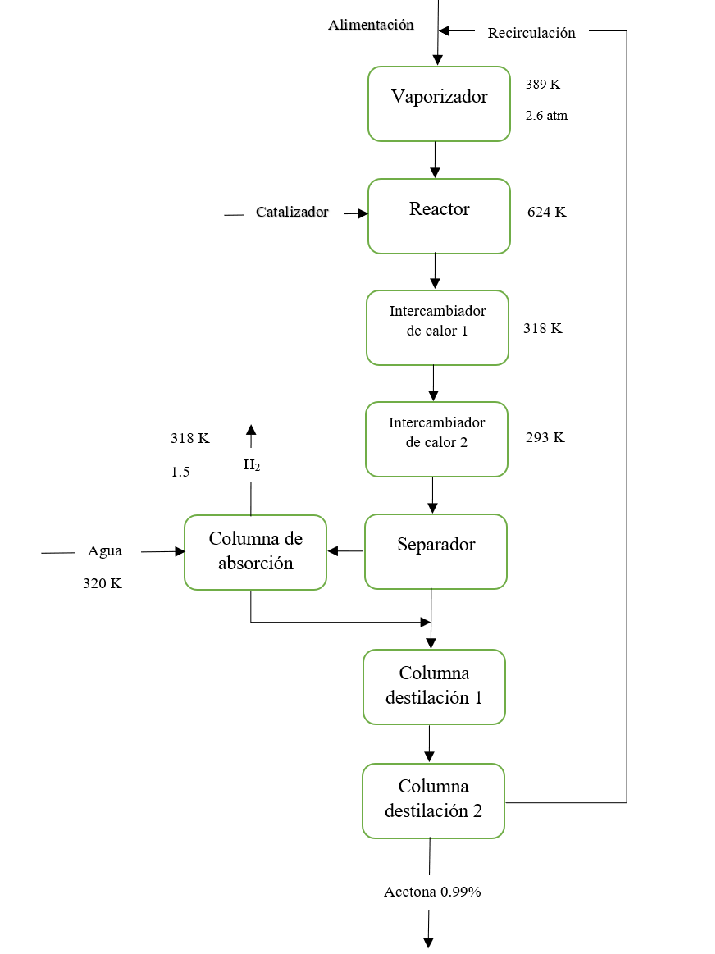
\includegraphics[scale=0.7]{images/Diagrama_completo.pdf}
            \caption{Diagrama de bloques del proceso}
            \label{fig:my_label}
        \end{figure}


\end{multicols}

    La principal ventaja de este proceso es que la acetona producida está libre de trazas de compuestos aromáticos, en particular benceno. Por esta razón la acetona producida a partir de alcohol isopropílico puede ser preferida por la industria farmacéutica, debido a las fuertes restricciones del uso de solventes.

    Al comienzo del proceso, la alimentación que contiene alcohol isopropílico y agua,  se mezcla con  la corriente de reciclaje  en el tambor de alimentación. Desde aquí, esta mezcla se envía al vaporizador, para cambiar la fase de la corriente como vapor. Después del vaporizador, la mezcla se calienta hasta la temperatura de reacción en el calentador.

    Acetona, hidrógeno gas $(H_2)$ se producen, y se descargan agua y alcohol isopropílico. La mezcla que son acetona, hidrógeno, agua y alcohol isopropílico se envían al enfriador y luego a un condensador. Después del condensador, la mezcla se envía al separador flash. Se obtiene hidrógeno, acetona, alcohol isopropílico y agua como producto superior. Este producto superior se envía a una torre de absorción para eliminar el hidrógeno. El producto inferior del separador flash que se compone de acetona, agua y alcohol isopropílico se mezclan con el producto de fondo de la columna de absorción antes de la primera columna de destilación. En esta, la acetona se obtiene del producto superior con 99\% en peso. La salida de la primera columna se envían a la segunda columna de destilación. Se envía el producto superior de la segunda columna para alimentar el tambor y el producto del fondo se desecha como agua residual \cite{article}.

    El la Figura \ref{fig:Diagrama} se muestra un diagrama  de proceso que muestra la ruta que sigue a través de los distintos equipos para la producción de acetona.
        \begin{figure}[H]
            \centering
            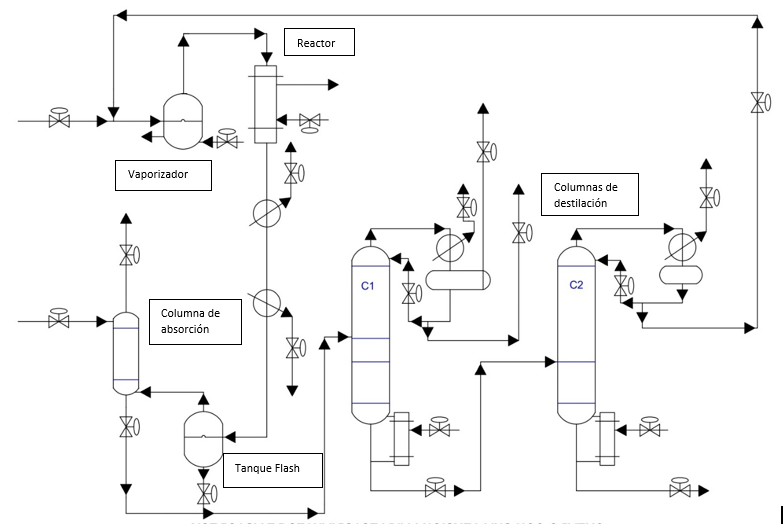
\includegraphics[scale = 0.55]{images/Diagrama_CAD.png}
            \caption{Diagrama del proceso.}
            \label{fig:Diagrama}
        \end{figure}

    \subsection*{Sistema de control}

    De las posibles opciones de control que existen dentro del sistema, se estudiaron las diversas posibilidades de los equipos de procesos y se toma la decisión de optar por la controlar la temperatura del reactor controlado la apertura de la válvula de  la chaqueta.
    \paragraph{}
    Para alcanzar los objetivos planteados en cuanto a obtener propuesta de control  es necesario tener en consideración el proceso dinámico del sistema. Para lograr el control automático de procesos se requiere del diseño e implementación de un
    sistema de control \cite{smith1991control}. Se debe considerar un objetivo de control. En este trabajo se plantea  como tal la temperatura del reactor . Se realizara mediante las ecuaciones descritas  anteriormente.
    La  reacción  del reactor  es:\\
                $$ A \rightarrow B +    C $$
    Donde $A$ es IPA, $B$ es la acetona  y $C$ es $H_2$\\
    Los balances de masa y energía  son:\\
        \begin{equation}
            \dfrac{dC_A}{dt}= r_A -\dfrac{F (C_{A0}-C_A)}{V}
            \label{balanceA}
        \end{equation}

        \begin{equation}
            \dfrac{dC_B}{dt}= -r_A +\dfrac{F(C_{B0}- C_B)}{V}
        \end{equation}

        \begin{equation}
            \dfrac{dC_C}{dt}= r_A +\dfrac{F(C_{C0} - C_C)}{V}
        \end{equation}

    Para el balance energía se tiene que:
        \begin{equation}
            \dfrac{dT_r}{dt} = \dfrac{F_r(T_f - T_r)}{V_r} + \dfrac{-\Delta H_{rxn}}{\rho_r C_{pr}}k_0exp\left(\frac{-E}{RT_r}\right)C_A -\dfrac{UA(T_r-T_j)}{V_r\rho_r C_{pr}}
            \label{energia}
        \end{equation}

        \begin{equation}
            \dfrac{dT_j}{dt} = \dfrac{F_j(T_{j0} - T_j)}{V_j}  +\dfrac{UA(T_r-T_j)}{V_j\rho_j C_{pj}}
            \label{energiachaqueta}
        \end{equation}

    Donde:

\begin{multicols}{2}
\paragraph{}

$C_A $ = Concentración de $A$\\
$C_B $ =Concentración de $B$\\
$C_C $ =Concentración de $C$\\
$C_{A0} $ =Concentración inicial de $A$\\
$C_{B0} $ =Concentración inicial de $B$\\
$C_{C0} $ =Concentración inicial de $C$\\
$U$ = Coeficiente global de transferencia de calor \\
$A$ = Área del intercambiador\\
$T_f$ = Temperatura de entrada\\
$T_j $ = Temperatura de la chaqueta\\
$F_r$ =  Flujo de entrada del reactor\\
$F_j$ =  Flujo de entrada  de la chaqueta\\
$ T_r $ =  Temperatura del reactor\\
$E $= Energía de activación\\
$R $= Constante de los gases ideales\\
$V_r $= Volumen de reactor\\
$V_j $= Volumen de la chaqueta\\
$ \rho_r $ = Densidad del flujo  de entrada al reactor\\
$ \rho_j $ = Densidad del flujo  de entrada a la chaqueta\\
$C_{pr}$= Capacidad calorífica del flujo de entrada al reactor\\
$C_{pj}$= Capacidad calorífica del flujo de entrada a la chaqueta\\
$ k_0$= Constante de reacción cinética \\
$\Delta H_{rxn}$ =  $\Delta H$ de reacción

\end{multicols}

\section*{Plan de trabajo}
    En cuanto al objetivo de  simulación del proceso es necesario  contar  con el software de Aspen  plus 10.0 además datos importantes como el modelado adecuado para satisfacer los parámetros necesarios que exige el simulador. Se necesita parámetros como flujos de entrada,temperatura de operación, presión de operación, composición de las corrientes de entrada y de salida además el modelo termodinámico. Los equipos cuya información es necesaria son:\\

        \begin{enumerate}
            \item Separador flash
            \item Reactor
            \item Intercambiadores de calor
            \item Torre de absorción
            \item Torres de destilación
        \end{enumerate}

    Los cuales los podemos encontrar en los distintas referencias de este trabajo.

    Para cumplir el objetivo de simular el proceso es necesario  iniciar un nuevo proyecto en blanco en Aspen 10.0, ingresar los componentes que se utilizaran en el desarrollo de la simulación, en este caso serán  necesarios Alcohol isopropilico ($C_3H_8O$), acetona ($C_3H_6O$ ), hidrógeno ($H_2$) y agua ($H_2O$), los cuales se ingresaran en el área de \textit{components} de la izquierda superior, además  se podrá añadir un nombre de reconocimiento de cada componente en este trabajo  para dar seguimiento a la simulación se dará el ID de \textit{ IPA},\textit{ ACETONE},\textit{ WATER} e \textit{ HYDROGEN}, tal
    como se muestra en la \textit{Figura \ref{fig:componentes}}.
        \begin{figure}[H]
            \centering
            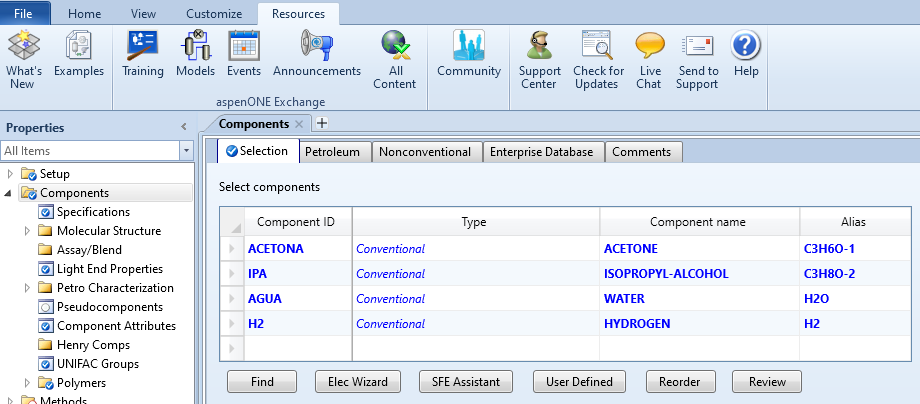
\includegraphics[scale =0.5]{images/Paso _1.PNG}
            \caption{Vista de Aspen Plus donde se introducen los componentes del proceso.}
            \label{fig:componentes}
        \end{figure}
    El siguiente paso es seleccionar el método con el que se va a trabajar, según la literatura  el método idóneo es UNIQUAC \cite{article}. El método anterior  toma en cuenta el tamaño molecular  y las diferencias de forma además de un termino residual que toma en cuenta las interacciones moleculares \cite{smith1997introduccion}, por lo tanto se especifica en la izquierda superior en el área de \textit{Methods} se selecciona UNIQUAC como en la \textit{Figura \ref{fig:Modelotermodinamico}}
        \begin{figure}[H]
            \centering
            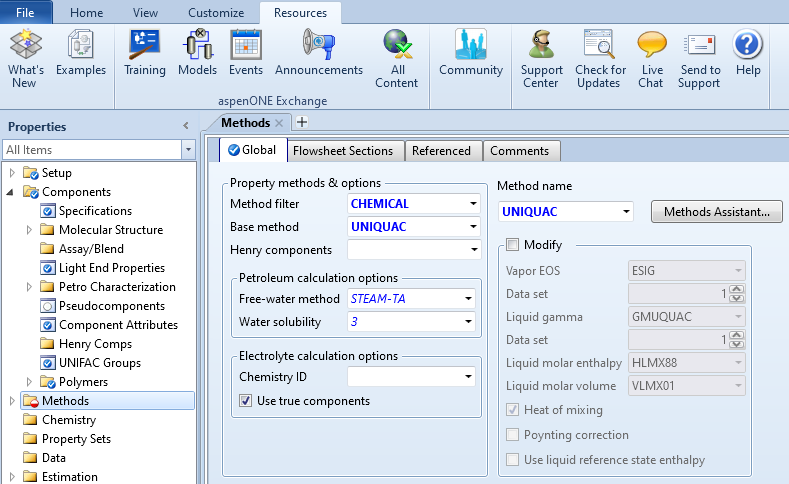
\includegraphics[scale=0.5]{images/Paso_2.PNG}
            \caption{Vista de Aspen Plus donde se muestra la selección del modelo termodinámico adecuado al proceso. Aquí se elige el modelo termodinámico UNIQUAC.}
            \label{fig:Modelotermodinamico}
        \end{figure}

    El área para  para insertar los reactores, a la izquierda inferior en el área \textit{simulation}\\ en el cual podemos escoger  entre diferentes tipos como RCSTR, Rplug, RBatch entre otros (ver\textit{ Figura \ref{fig:reactor}}).
        \begin{figure}[H]
            \centering
            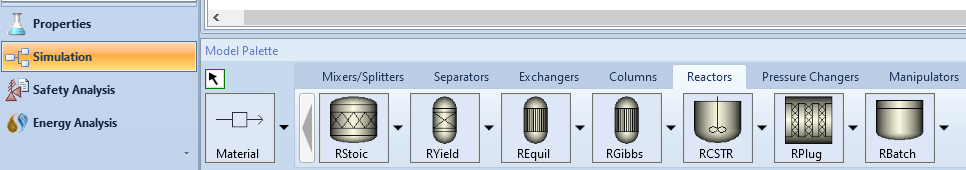
\includegraphics[scale=0.5]{images/Paso_3.PNG}
            \caption{Vista de Aspen Plus para la selección del reactor adecuado al proceso.}
            \label{fig:reactor}
        \end{figure}
    Para agregar la reacción en la sección de
    \textit{Reactions} en la cual agregaremos la reacción en ambos sentidos por ser reversible
        \begin{figure}[H]
            \centering
            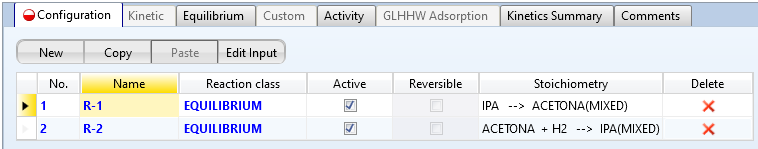
\includegraphics[scale=0.5]{images/Paso_4.PNG}
            \caption{Vista de Aspen Plus para la selección de parámetros cinéticos. Aquí seleccionamos si nuestra reacción es reversible o irreversible.}
            \label{fig:Parametrocineticos}
        \end{figure}
    Para agregar las columnas de destilación así como en el reactor, en la parte inferior  donde están las operaciones unitarias (ver\textit{ Figura \ref{fig:reactor}}) se selecciona  la pestaña de \textit{Columns} las columnas de destilación  y se llenan los datos necesarios como lo es la presión de operación que la literatura marca de 1 atm, la relación de reflujo que es de 2.78  y las distintas etapas necesarias así como la etapa  en la que se alimenta. En el proceso de Turton la primera columna tiene 67 etapas y se alimenta en la 54, para la segunda la columna tiene un total de 20 y se alimenta en la etapa 16 \cite{article}.

% Table generated by Excel2LaTeX from sheet 'Hoja1'
\begin{table}[htbp]
    \centering
    \caption{Add caption}
    \begin{turn}{90}
      \begin{tabular}{lr|rrrrrrrrrrrrrrrrrr}
      \toprule
            &       & \multicolumn{1}{l}{Feb} & \multicolumn{4}{c}{Mar}       & \multicolumn{5}{c}{Abr}               & \multicolumn{4}{c}{May}       & \multicolumn{4}{c}{Jun} \\
  \cmidrule{3-20}          &       & \multicolumn{1}{c}{26} & \multicolumn{1}{c}{5} & \multicolumn{1}{c}{12} & \multicolumn{1}{c}{19} & \multicolumn{1}{c}{26} & \multicolumn{1}{c}{2} & \multicolumn{1}{c}{9} & \multicolumn{1}{c}{16} & \multicolumn{1}{c}{23} & \multicolumn{1}{c}{30} & \multicolumn{1}{c}{7} & \multicolumn{1}{c}{14} & \multicolumn{1}{c}{21} & \multicolumn{1}{c}{28} & \multicolumn{1}{c}{4} & \multicolumn{1}{c}{11} & \multicolumn{1}{c}{18} & \multicolumn{1}{c}{25} \\
      \midrule
      Titulo &       & \cellcolor[rgb]{ .776,  .937,  .808}\textcolor[rgb]{ 0,  .38,  0}{} & \cellcolor[rgb]{ .776,  .937,  .808}\textcolor[rgb]{ 0,  .38,  0}{} &       &       &       &       &       &       &       &       &       &       &       &       &       &       &       &  \\
      \midrule
      \multicolumn{1}{c}{\multirow{2}[4]{*}{Objetivos}} & \multicolumn{1}{l|}{Generales} &       & \cellcolor[rgb]{ .776,  .937,  .808}\textcolor[rgb]{ 0,  .38,  0}{} &       &       &       &       &       &       &       &       &       &       &       &       &       &       &       &  \\
  \cmidrule{2-20}          & \multicolumn{1}{l|}{Especificos} &       & \cellcolor[rgb]{ .776,  .937,  .808}\textcolor[rgb]{ 0,  .38,  0}{} &       &       &       &       &       &       &       &       &       &       &       &       &       &       &       &  \\
      \midrule
      \multicolumn{1}{c}{\multirow{4}[8]{*}{Fundamentos}} & \multicolumn{1}{p{6.11em}|}{Descipción del proceso} &       &       & \cellcolor[rgb]{ .776,  .937,  .808}\textcolor[rgb]{ 0,  .38,  0}{} &       &       &       &       &       &       &       &       &       &       &       &       &       &       &  \\
  \cmidrule{2-20}          & \multicolumn{1}{p{6.11em}|}{Rutas de reacción} &       &       &       & \cellcolor[rgb]{ .776,  .937,  .808}\textcolor[rgb]{ 0,  .38,  0}{} &       &       &       &       &       &       &       &       &       &       &       &       &       &  \\
  \cmidrule{2-20}          & \multicolumn{1}{p{6.11em}|}{Diagrama de bloques} &       &       &       &       & \cellcolor[rgb]{ .776,  .937,  .808}\textcolor[rgb]{ 0,  .38,  0}{} &       &       &       &       &       &       &       &       &       &       &       &       &  \\
  \cmidrule{2-20}          & \multicolumn{1}{p{6.11em}|}{Propuesta de control} &       &       &       &       &       & \cellcolor[rgb]{ .776,  .937,  .808}\textcolor[rgb]{ 0,  .38,  0}{} &       &       &       &       &       &       &       &       &       &       &       &  \\
      \midrule
      Viabilidad &       &       &       &       &       &       &       & \cellcolor[rgb]{ .776,  .937,  .808}\textcolor[rgb]{ 0,  .38,  0}{} &       &       &       &       &       &       &       &       &       &       &  \\
      \midrule
      Estrategias &       &       &       &       &       &       &       &       & \cellcolor[rgb]{ .776,  .937,  .808}\textcolor[rgb]{ 0,  .38,  0}{} &       &       &       &       &       &       &       &       &       &  \\
      \midrule
      Cronograma &       &       &       &       &       &       &       &       &       & \cellcolor[rgb]{ .776,  .937,  .808}\textcolor[rgb]{ 0,  .38,  0}{} &       &       &       &       &       &       &       &       &  \\
      \midrule
      \multicolumn{1}{c}{\multirow{5}[10]{*}{Simulacion}} & \multicolumn{1}{l|}{Flash} &       &       &       &       &       &       &       &       &       & \cellcolor[rgb]{ .776,  .937,  .808}\textcolor[rgb]{ 0,  .38,  0}{} &       &       &       &       &       &       &       &  \\
  \cmidrule{2-20}          & \multicolumn{1}{l|}{Reactor} &       &       &       &       &       &       &       &       &       &       & \cellcolor[rgb]{ .776,  .937,  .808}\textcolor[rgb]{ 0,  .38,  0}{} &       &       &       &       &       &       &  \\
  \cmidrule{2-20}          & \multicolumn{1}{p{6.11em}|}{Intercambiador de calor} &       &       &       &       &       &       &       &       &       &       & \cellcolor[rgb]{ .776,  .937,  .808}\textcolor[rgb]{ 0,  .38,  0}{} &       &       &       &       &       &       &  \\
  \cmidrule{2-20}          & \multicolumn{1}{p{6.11em}|}{Torres de absorción} &       &       &       &       &       &       &       &       &       &       &       & \cellcolor[rgb]{ .776,  .937,  .808}\textcolor[rgb]{ 0,  .38,  0}{} &       &       &       &       &       &  \\
  \cmidrule{2-20}          & \multicolumn{1}{p{6.11em}|}{Torres de destilación} &       &       &       &       &       &       &       &       &       &       &       &       & \cellcolor[rgb]{ .776,  .937,  .808}\textcolor[rgb]{ 0,  .38,  0}{} &       &       &       &       &  \\
      \midrule
      Resultados &       &       &       &       &       &       &       &       &       &       &       &       &       & \cellcolor[rgb]{ .776,  .937,  .808}\textcolor[rgb]{ 0,  .38,  0}{} &       &       &       &       &  \\
      \midrule
      \multicolumn{1}{p{5.39em}}{Viabilidad sustentable} &       &       &       &       &       &       &       &       &       &       &       &       &       &       & \cellcolor[rgb]{ .776,  .937,  .808}\textcolor[rgb]{ 0,  .38,  0}{} &       &       &       &  \\
      \midrule
      Concluciones &       &       &       &       &       &       &       &       &       &       &       &       &       &       &       & \cellcolor[rgb]{ .776,  .937,  .808}\textcolor[rgb]{ 0,  .38,  0}{} & \cellcolor[rgb]{ .776,  .937,  .808}\textcolor[rgb]{ 0,  .38,  0}{} & \cellcolor[rgb]{ .776,  .937,  .808}\textcolor[rgb]{ 0,  .38,  0}{} &  \\
      \midrule
      Presentación &       &       &       &       &       &       &       &       &       &       &       &       &       &       &       &       &       &       & \cellcolor[rgb]{ .776,  .937,  .808}\textcolor[rgb]{ 0,  .38,  0}{} \\
      \bottomrule
      \end{tabular}%
    \end{turn}
    \label{tab:addlabel}%
  \end{table}%
  

%======================================%
%           Referencias                %
%======================================%
%\printbibliography

\bibliographystyle{apacite}
%\bibliographystyle{newapa}
\bibliography{referencias.bib}

\end{document}
